\documentclass[10pt]{beamer}

\usetheme[progressbar=frametitle]{metropolis}
\usepackage{appendixnumberbeamer}

\usepackage{booktabs}
\usepackage[scale=2]{ccicons}
\usepackage{diagbox}
\usepackage{pifont}
\newcommand{\cmark}{\ding{51}}
\newcommand{\xmark}{\ding{55}}

\usepackage{pgfplots}
\usepgfplotslibrary{dateplot}
\usepackage{amssymb,amsmath}

\usepackage{tikz}
\usetikzlibrary{positioning}

\usepackage{xspace}
\usepackage{multirow}
\usepackage[ruled, linesnumbered]{algorithm2e}
\usepackage{multimedia}
\usepackage{media9}
\newcommand{\includemovie}[3]{%
\includemedia[%
width=#1,height=#2,%
activate=pagevisible,%
deactivate=pageclose,%
addresource=#3,%
flashvars={%
src=#3 % same path as in addresource!
&autoPlay=true % default: false; if =true, automatically starts playback after activation (see option ‘activation)’
&loop=true % if loop=true, media is played in a loop
&controlBarAutoHideTimeout=0 %  time span before auto-hide
}%
]{}{StrobeMediaPlayback.swf}%
}% end of the new command

% For caption without labels
\usepackage{caption}
\setbeamertemplate{caption}{\raggedright\insertcaption\par}

\newcommand{\lv}{\lVert}
\newcommand{\rv}{\rVert}

\AtBeginSection{%
\begin{frame}
    \tableofcontents[currentsection, subsectionstyle=show/show/hide]
\end{frame}
}


\title{CXPlain: Causal Explanations for Model Interpretation under Uncertainty}

\date{Apr 27, 2020}
\author[Patrick Schwab and Walter Karlen]{Patrick Schwab and Walter Karlen \\[5pt]
\small{Presented by Chuan Lu and Chengyue Huang}}


\titlegraphic{\vspace{5cm}\flushright
\includegraphics[width=2cm,height=2cm]{figures/DomeWordPrimaryBLACK.eps}}

\begin{document}

\maketitle

\begin{frame}
\tableofcontents
\end{frame}

\section{Introduction and Related Work}

\begin{frame}{Introduction}
\begin{itemize}
\item Explanation methods for machine learning models are important, but complex models are difficult to interpret
\item Wide variety of machine learning models make it challenging to develop a fast, accurate, unified and optimized approach to importance attribution for any machine learning models
\item State-of-the-art explanation methods typically have significant uncertainty, difficult to judge if the explanation results are accurate

\end{itemize}
\end{frame}

\begin{frame}{Drawbacks of Existing Methods}
\textbf{Computational cost and Applicability}
\begin{figure}
\centering
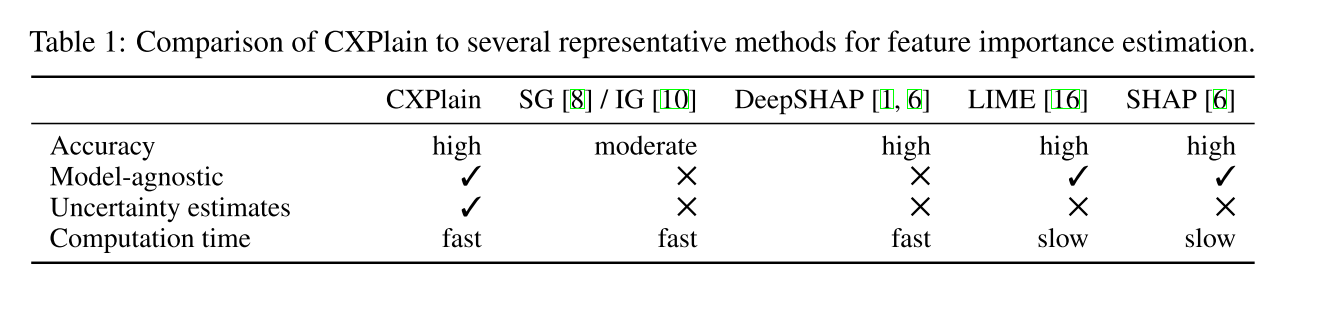
\includegraphics[width=\textwidth]{figures/introduction/table1.png}
\end{figure}
\end{frame}

\begin{frame}{Drawbacks of Existing Methods}
\textbf{Uncertainty in explanation}
\begin{figure}
\centering
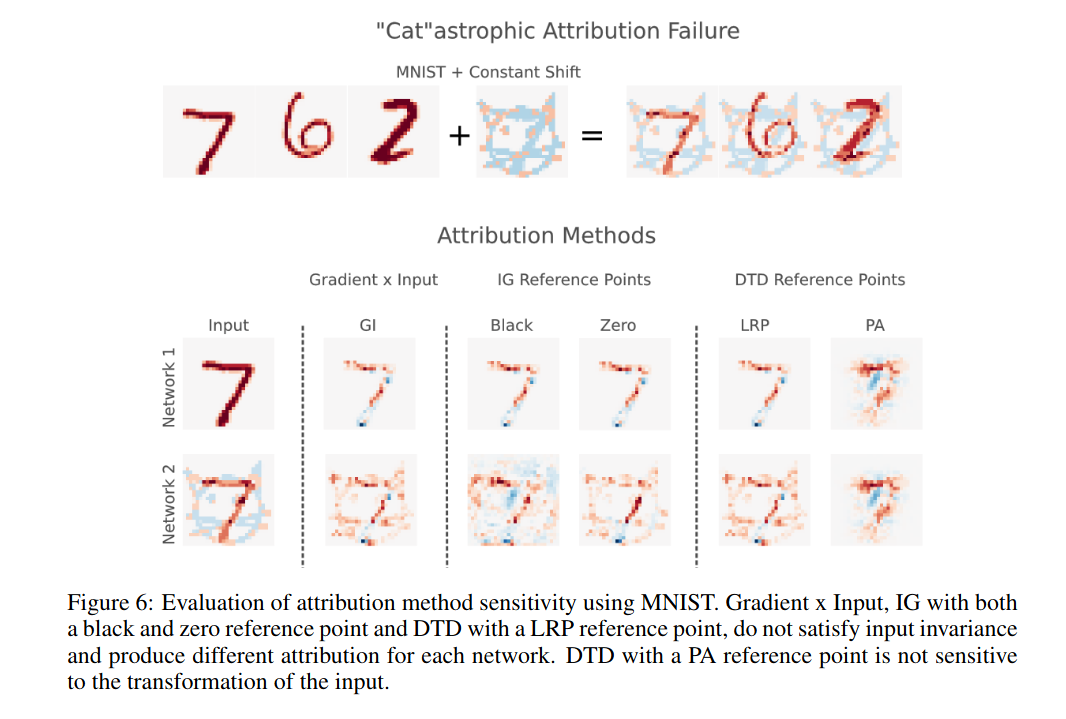
\includegraphics[width=.95\textwidth]{figures/introduction/uncertainty1.png}
\footnotemark[1]
\end{figure}
\footnotetext[1]{\tiny Pieter-Jan Kindermans, Sara Hooker, Julius Adebayo, Maximilian Alber, Kristof T Schütt, Sven Dähne, Dumitru Erhan, and Been Kim. The (un) reliability of saliency methods. arXiv preprint arXiv:1711.00867, 2017.}
\end{frame}

\begin{frame}{Drawbacks of Existing Methods}
\begin{figure}
\centering
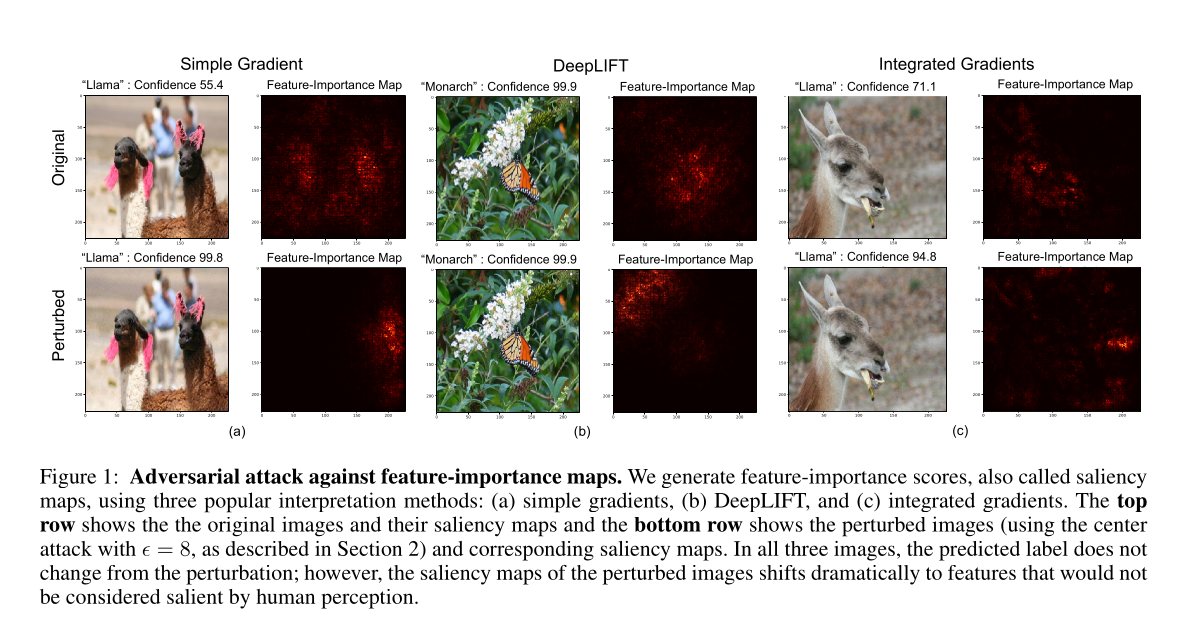
\includegraphics[width=.95\textwidth]{figures/introduction/uncertainty2.png}
\footnotemark[2]
\end{figure}
\footnotetext[2]{\tiny Amirata Ghorbani, Abubakar Abid, and James Zou. Interpretation of neural networks is fragile. AAAI Conference on Artificial Intelligence, 2019.}
\end{frame}

\begin{frame}{CXPlain}
\begin{itemize}
\item Causal Explanation Model
\item Estimate feature importance for \textbf{any} machine learning model
\item Significantly \textbf{more accurate} and \textbf{faster} in evaluation than existing model-agnostic methods
\item Provide uncertainty estimates for feature importance by bootstrap resampling
\item Uncertainty estimates are strongly correlated with the accuracy of the explanation model
\end{itemize}

Idea: train a seperate explanation model to produce the importance scores for each input features.
\end{frame}

\begin{frame}
\centering
\Huge Questions?
\end{frame}


\section{Methodology}
\begin{frame}{Problem Setup}

\textbf{Predictive model}

\begin{itemize}
\item Suppose we have a predictive model $\hat{f}: X \to \hat{y}\in\mathbb{R}^{k}$, where $X$ consists of $p$ input features $\{x_i\}_{i=1}^{p} $

\item The predictive model is scored by an objective function $\mathcal{L}$

\item No other restrictions on $\hat{f}$, no need for knowledge on how $\hat{f}$ produces its output

\end{itemize}

\textbf{Explanation model}
\begin{itemize}
\item Goal: train an explanation model $\hat{f}_{exp}: X\to \hat{A}\in \mathbb{R}^p $, where each element $\hat{a}_i $ corresponds to the importance score of input feature $x_i $.
\end{itemize}

\begin{figure}
\centering
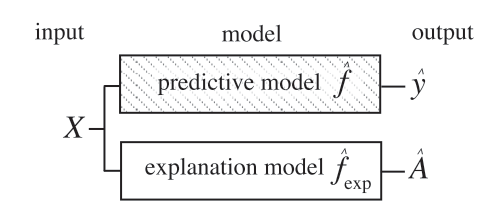
\includegraphics[width=.5\textwidth]{figures/methodology/model structure.png}
\end{figure}
\end{frame}

\begin{frame}{Causal Objective}
Given input features $X$, we compute the outputs of the predictive model $\hat{f}$ with and without the $i$th input feature $x_i $:
\begin{equation}
\hat{y}_{X\setminus\{i\}} = \hat{f}(X\setminus \{i\}), \quad \hat{y}_{X} = \hat{f}(X)
\end{equation}

Then we compute the errors of the predictive model $\hat{f}$ with and without $x_i $ using the loss function $\mathcal{L}$ of $\hat{f}$:
\begin{equation}
\varepsilon_{X\setminus\{i\}} = \mathcal{L}(y, \hat{y}_{X\setminus\{i\}}), \quad \varepsilon_{X} = \mathcal{L}(y, \hat{y}_X)
\end{equation}

The \textbf{causality} of input feature $x_i $ to model output $y$ is defined as the \textbf{marginal decrease} in the predictive error:
\begin{equation}
\Delta\varepsilon_{X, i} = \varepsilon_{X\setminus\{i\}} - \varepsilon_{X}
\end{equation}
\end{frame}

\begin{frame}{Causal Objective}
We get the \textbf{importance scores} by normalizing the causalities:
\begin{equation}
\omega_i(X) = \frac{\Delta\varepsilon_{X, i}}{\sum_{j=1}^{p}\Delta\varepsilon_{X, j}}
\end{equation}

Finally, we define the \textbf{causal objective} as the Kullback-Leibler divergence between the target importance distribution $\Omega$ and the one computed by the explanation model:
\begin{equation}
\mathcal{L}_{\text{causal}} = \frac{1}{N}\sum_{l=1}^{N}\text{KL}(\Omega_{X_l}, \hat{A}_{X_l}),
\end{equation}
where $\Omega(i) = \omega_i(X)$, and $\hat{A}(i) = \hat{a}_i$ are the output of $\hat{f}_{exp} $.

\end{frame}


\begin{frame}{Remarks}

\textbf{Mask input features}
\begin{itemize}
\item Replace $x_i $ with zeros when the zero value has no special meaning
\item Replace $x_i $ with mean value across the entire dataset
\item Advanced schemes considering the distribution of the features can be more principled alternatives
\end{itemize}

\textbf{Precompute importance scores}
\begin{itemize}
\item To precompute the importance score for one training sample $X$ with $p$ features, $p+1$ evaluations of the predictive model are required
\item For high-dimensional images, we can group non-overlapping regions of adjacent pixels into feature groups
\end{itemize}
\end{frame}

\begin{frame}{Remarks}

\textbf{CXPlain models}
\begin{figure}
\centering
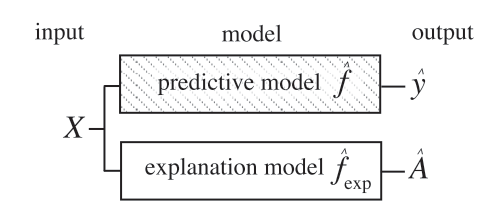
\includegraphics[width=.5\textwidth]{figures/methodology/model structure.png}
\end{figure}

\begin{equation}
\hat{f}_{\exp}: X = (x_1, x_2, \hdots, x_p) \to (\omega_1(X), \omega_2(X), \hdots, \omega_p(X))
\end{equation}

\begin{itemize}
\item Any supervised machine learning model that can be trained with a custom objective can be used as explanation models
\item In this work, the authors use DNNs, specifically MLPs and U-nets
\end{itemize}
\end{frame}

\begin{frame}{Uncertainty Quantification}

The uncertainty associated in feature importance estimate $\hat{a} $ can be quantified via bootstrap ensemble methods.
\begin{itemize}
\item Randomly draw $N$ training samples $X$ with repeats from the original training set (of size $N$), and train an explanation model on the selected set.
\item Repeat the process $M$ times to obtain a bootstrap ensemble of $M$ explanation models.
\item Use the median of the outputs as the assigned output, and use the $\frac{\alpha}{2}$ and $1-\frac{\alpha}{2}$ quantiles to form the confidence intervals $\text{CI}_{\gamma} = [c_{\frac{\alpha}{2}}, c_{1-\frac{\alpha}{2}}]$ at confidence level $\gamma = 1-\alpha$.
\item The width of $\text{CI}_{\gamma} $ can be used to quantify the uncertainty of $\hat{a} $.
\end{itemize}
\end{frame}

\begin{frame}
\centering
\Huge Questions?
\end{frame}

\section{Experiments}

\begin{frame}{Questions to answer}
\begin{itemize}
\item How does the feature importance estimation performance of CXPlain compare to that of the state-of-the-art methods? (Accuracy)
\item How does the computational performance of CXPlain compare to existing model-agnostic and model-specific methods for feature importance estimation? (Computational cost)
\item Are uncertainty estimates of CXPlain models qualitatively and quantitatively correlated with their ability to accurately determine feature importance? (Quality of uncertainty quantification)
\end{itemize}
\end{frame}

\begin{frame}{Tasks}
\textbf{Binary classification tasks:}
\begin{itemize}
\item 8 vs. 3 MNIST benchmark (model accuracy: 99.85\%)
\item Gorilla vs. Zebra ImageNet benchmark (model accuracy: 96.73\%)
\item The test set contains 100 unseen images
\end{itemize}
\begin{figure}
\centering
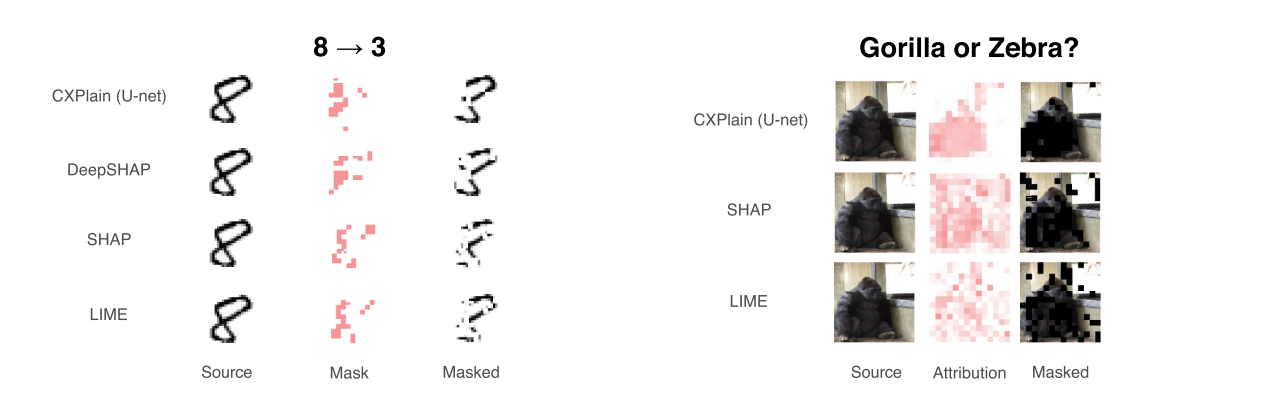
\includegraphics[width=\textwidth]{figures/experiment/tasks.png}
\end{figure}
\end{frame}

\begin{frame}{Metrics}
\textbf{Accuracy of important features}
\begin{itemize}
\item To quantify the accuracy of important features predicted, we measure the change in the classification models' confidence after masking the top 10 and 30\% of the most importanct pixels for MNIST and ImageNet test images respectively:
\begin{equation}
\Delta\text{log-odds} = \text{log-odds}(p_{\text{original}}) - \text{log-odds}(p_{\text{masked}})
\end{equation}
\item $\text{log-odds}(p) = \log\left(\frac{p}{1-p}\right)$
\item Higher $\Delta\text{log-odds}$ means higher accuracy in important feature estimation
\item Mann-Whitney-Wilcoxon (MWW) tests are used to calculate $p$-values for comparison between distributions.
\end{itemize}
\end{frame}

\begin{frame}{Metrics}
\textbf{Uncertainty Quantification}
\begin{itemize}
\item We want to test whether the uncertainty estimates $u_i $ of input feature $x_i $ are correlated with the errors in feature importance estimation on test set. That is to say, whether a small uncertainty provided by the ensemble models leads to a high accuracy in the estimation of importance scores.

\item The authors state that typically the per-feature ground-truth values of importance scores are not available, so the Rank Error $$\text{RE}_i = |\text{rank}_{\Delta\text{log-odds}}(i) - \text{rank}_{\hat{f}_{exp}}(i)| $$
defined as the difference in the rank of feature $x_i $ implied by $\Delta\text{log-odds}$ and the rank implied by $\hat{f}_{exp} $ is used as the error in importance estimation.
\end{itemize}
\end{frame}

\begin{frame}{Metrics}
\textbf{Uncertainty Quantification}
\begin{itemize}
\item Pearson correlation coefficient $\rho_{X, Y} = \frac{\text{cov}(X, Y)}{\sigma_X\sigma_Y} $ is used to measure the correlation between $\text{RE}_i $ and $u_i$
\item The coefficient $\rho$ is computed on the top $2.5\%$ of pixels by $\Delta\text{log-odds}$ across the test set of $N=100$ images.
\item Fisher $z$-transform is applied to the correlation scores to correct the skew in the distribution of sample correlation.
\end{itemize}
\end{frame}

\begin{frame}{Results}

\end{frame}

\section{Conclusion}


\end{document}